
\subsection{Invariance properties of $H$}
Recall that the physical space (determined by the Gauss law) is given by
	\[
	P = \Sp ( |n_0\, n_1\, \ldots \, n_{N-1} \, b_{-1}\, b_0\, \ldots\, b_{N-2}\rangle \ | \ b_{\ell} =b_{\ell-1} + n_{\ell} + \frac{1}{2}((-1)^\ell-1) \ \text{for every} \ \ell).
	\]
	We can split $P$ into the direct sum according to what value of $b_{-1}$ is:
	\[
	P = P_0 \oplus P_1 \oplus \cdots \oplus P_{n-1},
	\]
	where
	\[
	P_j = \Sp( |n_0\, n_1\, \ldots \, n_{N-1} \, b_{-1}\, b_0\, \ldots\, b_{N-2}\rangle \in P \ | \ b_{-1} = j).
	\]

Also, let $N:= \sum_{l} \psi_l^\dagger \psi_l$ be the operator that counts fermions.

The following lemma is an obvious but very useful observation:

\begin{lemma}\emph{(Invariance properties of $H$)} The following hold:
\begin{enumerate}[(i)]
\item The restriction of $H$ to each subspace $P_j$. Denote $H_j := H|_{P_j}$.
\item $[N,H] = 0$. In particular, for a chosen $|\gs\rangle$, the basic kets $|\psi\rangle$ for which $\langle \psi | \gs \rangle \neq 0$ all have the same number of fermions.
\end{enumerate}
\end{lemma}
\subsection{Dependence on $m$}
\begin{proposition}\label{p:dep_m}
Let $\lambda_1$ be the eigen-value of $H$ that corresponds to a ground state. Then $\lambda_1$ is a concave $C^1$-function of the mass. 
\end{proposition}
\begin{proof}
Concavity is a consequence of Proposition \ref{p:conv_le}; differentiability of $\lambda_1$ is a consequence of Theorem \ref{thm:pert}.
\end{proof}

\noindent \textbf{Caution:} one cannot choose ground states continuously (with respect to the mass). It's easy to see for odd $N$ (say, $N=3$): take limits $m\rightarrow \pm \infty$ and see that the number of fermions is not preserved. If a continuous choice was possible, it would be preserved. Also, a theorem that guarantees continuity of eigen-vectors requires holomorphicity of $H$ (see \cite{kato}, p. 121). The Hamiltonian is indeed holomorphic, but for complex values of $m$ it's not Hermitian, so that theorem is not applicable.
\subsection{Wilson loop for $m \gg 0$}
Split the Hamiltonian as $H = A + 2m\sqrt{n/2\pi} D$, where $A$ is the sum of the first term and the third terms of $H$ and $D = \sum_l (-1)^l \psi_l^\dagger \psi_l$.

\subsubsection{Estimate for $\lambda_1$}
\begin{proposition}\label{p:lambda_est_pos}
Let $\lambda_1$ be the eigen-value of $H$ that corresponds to a ground state. Then
\[
\lim_{m \rightarrow \infty} \frac{\lambda_1}{m} = -2\left[\frac{N}{2}\right]\sqrt{\frac{n}{2\pi}}.
\]
Also, for $m > 0$,
\[
\lambda_1(m) < -2m\left[\frac{N}{2}\right]\sqrt{\frac{n}{2\pi}}
\]
(note: the inequality is strict!). The limit implies that for $m \gg 0$ and $N$ even (or large), the lowest energy level can be approximated as 
\[
\lambda_1(m) \approx - Nm \sqrt{\frac{n}{2\pi}}.
\]
\end{proposition}
\begin{proof}
Let $m > 0$. From the definition of $|\gs\rangle$, we see that
\[
m^{-1}\langle \st_2(s) | H| \st_2(s) \rangle \geq m^{-1}\langle \gs | H| \gs \rangle = m^{-1}\min_{\|\psi\|=1} \langle \psi |H|\psi\rangle \geq m^{-1}\min_{\|\psi\|=1} \langle \psi |A |\psi\rangle + 2\sqrt{\frac{n}{2\pi}} \langle \st_2(s) | D| \st_2(s)\rangle 
\]
%Note that 
%\[
%\lim_{m\rightarrow \infty} m^{-1}\langle \st_2(s) | H|\st_2(s) \rangle = 2\sqrt{\frac{n}{2\pi}} \langle \st_2(s) | D| \st_2(s)\rangle
%\]
%and
Note that
\[
\langle \st_2(s) | H|\st_2(s) \rangle = 2m\sqrt{\frac{n}{2\pi}} \langle \st_2(s) | D + \sum_l E_{l,l+1}^2 | \st_2(s)\rangle = -2m\left[\frac{N}{2}\right]\sqrt{\frac{n}{2\pi}}
\]
so, taking the limit in the above series of inequalities, we obtain the result.
%Hence, taking the limit in the above inequality, we obtain the statement. With regards to $\lambda_1$, we write $\langle \gs | H| \gs \rangle = \lambda_1\langle \gs |\gs\rangle = \lambda_1$.
With regards to the strict inequality for $\lambda_1$, $|\st_2(s)\rangle$ is clearly not an eigen-value of $H$ when $m$ is finite, so $\langle\st_2(s)|H|\st_2(s)\rangle$ cannot equal $\lambda_1$ (see the footnote\footnote{Let $|\psi_k\rangle$ constitute an orthonormal basis of eigen-vectors of $H$ (they can be chosen to have real components with respect to the standard basis for $H$ is hermitian and symmetric). Then $|\st_2(s)\rangle = \sum_{k} \alpha_k |\psi_k\rangle$ and $\sum_{k}\alpha_k^2 = 1$ (all $\alpha_k$'s are real). On the other hand, applying $\langle \st_2 |H$ to both sides yields $\lambda_1 = \sum_{k} \alpha_k^2 \lambda_k$. Since $|\st_2(s)\rangle$ is not an eigen-vector of $H$, there's $\lambda_j > \lambda_1$ such that $\alpha_j \neq 0$. We want to show that the above equality is not possible. Indeed, let $m$ be the index of the last $\lambda_i$ that is equal to $\lambda_1$. We can rewrite the equation as $\lambda_1 = \sum_{k=m+1}^n \frac{\alpha_k^2}{1-\sum_{i=1}^m \alpha_i^2} \lambda_k$, which is again a convex combination, so write $\lambda_1 = \sum_{k=m+1}^n \beta_k\lambda_k$. We know that $\lambda_1 < \lambda_{k}$ for every $k> m$. But then $\beta_k\lambda_1 \leq \beta_k\lambda_k$ for $k > m$, and for $j$ the inequality is strict: $\beta_j\lambda_1 < \beta_j\lambda_j$; summing up, we get $\sum_{k=m+1}^n \beta_k\lambda_1 < \sum_{k=m+1}^n \beta_k \lambda_k$, which contradicts the equality. Thus $\lambda_1 \neq \langle \st_2(s)|H|\st_2(s)\rangle$.

} for a detailed theoretical explanation).
\end{proof}
\noindent \textbf{Remark.} Notice that L'Hopitals rule gives us an estimate for the derivative $\lambda_1^\prime$ with respect to $m$:
\[
\lim_{m \rightarrow \infty} \lambda_1^\prime(m) = -2\left[\frac{N}{2}\right] \sqrt{\frac{n}{2\pi}}.
\]

\noindent\emph{How good is the estimate?} Let me show on a chart with random data ($N= 6$ and $n= 7$). The graphed function is $m \mapsto 2m[N/2]\sqrt{n/(2\pi)} - \lambda_1(m)$.
\begin{center}
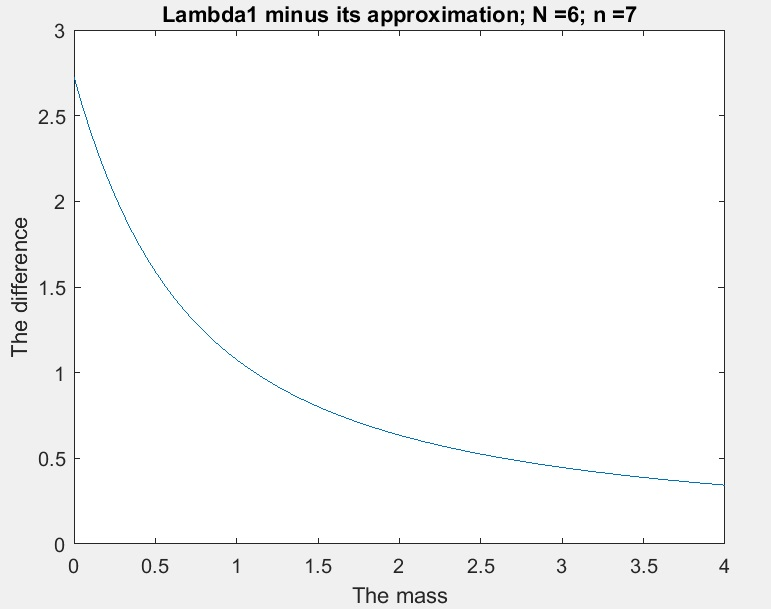
\includegraphics[scale=0.8]{conv6_7.jpg}
\end{center}


\subsubsection{Ground states}

\begin{lemma} \label{l:gs_conv_pos}
The following hold:
\begin{enumerate}
\item For any basic ket $|\psi\rangle$ such that $\langle \psi |D|\psi\rangle > -[N/2]$ (i.e., $|\psi\rangle \neq |\st_2(i)\rangle$ for any $i$), we have $\lim_{m \rightarrow \infty} \langle \gs | \psi \rangle = 0$;
\item For\footnote{By this I mean that there exists $m_0 > 0$ such that for all $m \geq m_0$ the statement is true.} $m \gg 0$ we have $\left\langle \gs | \st_2(s) \right\rangle \neq 0$. In particular, if for every large enough mass we choose $|\gs\rangle$ so that $\langle \gs | \st_2(s) \rangle > 0$ (which is possible), then $\lim_{m \rightarrow \infty} |\gs\rangle = |\st_2(s)\rangle$. 
\item As a consequence of the above, for $m \gg 0$, $|\gs\rangle \in P_s$, and the number of fermions in each non-zero component of $|\gs\rangle$ is equal to $[N/2]$.
\end{enumerate}
\end{lemma}
\begin{proof}
\begin{enumerate}
\item Indeed, we see that
\[
\langle \psi | \gs \rangle = \frac{1}{\lambda_1} \langle \psi | H|\gs\rangle = \frac{1}{\lambda_1} \langle \psi |A|\gs\rangle + \frac{2m}{\lambda_1} \sqrt{\frac{n}{2\pi}} \langle \psi | D | \gs \rangle = \frac{1}{\lambda_1} \langle \psi |A|\gs\rangle + \frac{2m}{\lambda_1} \sqrt{\frac{n}{2\pi}} \cdot a \langle \psi | \gs \rangle
\]
where $a$ is an eigen-value of $D$ (which is not equal to $-[N/2]$ by assumption). The above can be rewritten as
\[
\langle \psi | \gs\rangle = \frac{1}{\lambda_1} \frac{1}{1- \frac{2ma}{\lambda_1}\sqrt{\frac{n}{2\pi}} } \langle \psi | A | gs\rangle.
\]
We see that 
\[
1- \frac{2ma}{\lambda_1}\sqrt{\frac{n}{2\pi}} \rightarrow 1 + a [N/2]^{-1} \neq 0
\]
therefore
\[
\lim_{m \rightarrow \infty}\langle \psi | \gs \rangle = 0.
\]
\item Since each $P_i$ is invariant under $H$, we find $j$ such that $|\gs \rangle \in P_j$, so we can write it as $|\gs\rangle = \alpha |\st_2(j)\rangle + |v\rangle$, where $|v\rangle \perp |\st_2(j)\rangle$. Together with $\langle \gs | \gs \rangle = 1$, the above implies
\[
\lim_{m \rightarrow \infty} (1 - |\alpha|^2) = 0
\]
or $\lim_{m \rightarrow \infty} |\langle \gs |\st_2(j)\rangle| = 1$. If we made the choice of ground states so that $\alpha > 0$, then $\lim_{m\rightarrow \infty} \alpha = 1$, so $|\gs\rangle \rightarrow |\st_2(j)\rangle$.

Let's prove that $j = s$. Write $|\gs\rangle = \alpha |\st_2(j)\rangle + \beta |v\rangle$ and $|\gs^\prime\rangle = \alpha |\st_2(s)\rangle + \beta |v^\prime \rangle$. The vector $|v^\prime \rangle$ is totally the same as $|v\rangle$ except that we substitute everywhere the bosonic state $b_{-1} = j$ with the state $b_{-1} = s$. The constants $\alpha$ and $\beta$ can be chosen real, $\alpha > 0$, and $\alpha^2+\beta^2 = 1$. Then we compare the expectation values of the Hamiltonian:
\[
\langle \gs | H|\gs \rangle  = \alpha^2 (-2m[N/2] \sqrt{n/2\pi} + (N-1)(j-s)^2) + O(\beta),
\]
\[
\langle \gs^\prime | H|\gs^\prime \rangle  = \alpha^2 (-2m[N/2] \sqrt{n/2\pi}) + O(\beta),
\]
hence their difference is
\[
\langle \gs | H|\gs \rangle - \langle \gs^\prime | H|\gs^\prime \rangle = \alpha^2(N-1)(j-s)^2 + O(\beta).
\]
It is supposed to be always negative. However, we can make $O(\beta)$ as small as we want, whereas $\alpha^2$ tends to $1$ and is multiplied by something stubbornly positive. Therefore, the difference can stay negative iff $j = s$.
\end{enumerate}
\end{proof}

\begin{conj}
It is true for any $m > 0$ that $\langle \gs|\st_2(s)\rangle \neq 0$. Numerical experiments suggest even more: $\langle \gs | \st_2(s)\rangle > \langle \gs | \psi \rangle$ for any other basic ket $\psi$.
\end{conj}

%\begin{proposition}
%We have $|\gs\rangle \in P_s$ for \emph{any} $m$, and $N|\gs\rangle = [N/2] |\gs\rangle$.
%\end{proposition}
%\begin{proof}
%This is pure general topology. For any fixed ground state at a particular mass, we can find a $C^1$-curve $m \mapsto |\gs\rangle$ that passes through it. The image of the ground state curve lies in the disjoint union $P_1 \cap S^{\dim P} \cup \cdots \cup P_n \cap S^{\dim P}$. Since $|\gs\rangle$ is in particular continuous in $m$, the image of $\mathbb R$ lies only in one of the components of the union. Since for $m \gg 0$ it happens in $P_s\cap S^{\dim P}$, it's there for \emph{any} $m$.
%\end{proof}

\begin{proposition}\label{p:large_mass_nondeg}
For $m \gg 0$, a ground state is non-degenerate.
\end{proposition}
\begin{proof}
Assume on the contrary that it is degenerate for $m \gg 0$. This means there's a sequence of values of mass $m_k \rightarrow \infty$ and sequences of ground states $|\gs_k\rangle$ and $|\gs^\prime_k\rangle$ such that $\langle\gs_k^\prime|\gs_k\rangle = 0$. However, passing to the limit in the slots of the Hermitian product yields $\langle \st_2(s) | \st_2(s) \rangle \neq 0$. This is a contradiction, and thus the ground state is unique for large $m$.
\end{proof}
%\begin{proof}[Heuristic evidence]
%I believe that $|\gs\rangle$, if chosen so that $\langle \gs | \st_2(s)\rangle \in [0,1]$, is a continuous function of $m$. The eigen-value $\lambda_1$ is continuous as well. But recall that $P = P_1 \oplus \cdots \oplus P_n$. The sets $S^{\dim P} \cap P_i$ (an intersection of the unit sphere with a subspace) are disjoint, and since $|\gs\rangle$ is continuous, it maps the whole real line $\mathbb R$ into only one such intersection, i.e. into $S^{\dim P} \cap P_s$. So $b_{-1} = s$ always has to be the bosonic state for $|\gs\rangle$.
%\end{proof}

\begin{proposition}
Let $\Sigma = N^{-1}\sum \langle E_{l,l+1} \rangle$ be the electric field operator. Then\footnote{No matter how we choose the ground states for every value of mass since we're under the Hermitian inner product.} $\lim_{m \rightarrow \infty} \Sigma = 0$.
\end{proposition}
\begin{proof}
Indeed, by Lemma \ref{l:gs_conv_pos} we can assume that $\lim_{m \rightarrow \infty} |\gs\rangle = |\st_2(s)\rangle$. Then 
\[
\langle \gs | E_{l,l+1} | \gs \rangle \rightarrow \langle \st_2(s) | E_{l,l+1}|\st_2(s)\rangle = 0.\qedhere
\]
\end{proof}

\subsubsection{Non-degeneracy of $|\gs\rangle$}

We proved in the previous subsubsection that the ground state is non-degenerate for $m \gg 0$. There is also a different way to state non-degeneracy for an arbitrary mass but with making a natural assumption with regards to the ground state. This assumption holds in numerical examples for positive mass (for $N$ odd and $m < 0$ the number of fermions is different), so the condition is applicable in principle.

\begin{proposition}
Assume that $|\gs\rangle \in P_s$ and the number of fermions in $|\gs\rangle$ is equal to $[N/2]$. Then the ground state is non-degenerate if
\[
\frac{n}{2\pi}\left(2N-3\right) < 4m \sqrt{\frac{n}{2\pi}} + 1.
\]
\end{proposition}
Assuming $N \gg 0$, this can be restated as (only approximately, non-rigorously) 
\[
\frac{N \sqrt{n}}{m} < \sqrt{8\pi}.
\]
At least this gives the order of contribution for each parameter. It also gives another proof of the fact that the ground state is non-degenerate when the mass is large enough, and we have a sufficient estimate for that mass. \emph{Practically speaking, the estimate is useless; the point, I think, is only to show that Gershgorin's theorem is not handy in our case.}
\begin{proof}
The sufficient condition can be derived from Gershgorin's theorem (see appendix). We consider the Hamiltonian restricted to the subspace with $b_{-1} = s$ and with the number of fermions equal to $[N/2]$. Let $D_1$ and $D_2$ be respectively the leftmost and the rightmost Gershgorin intervals. Note the following: $D_1$ is centered at the value corresponding to $|\st_2(s)\rangle$, and the center of $D_2$ to the value corresponding to $|\st_2(s)\rangle$ with any fermion hopped to a nearby site. Then $D_1$ is centered at $-2m[N/2]\sqrt{n/(2\pi)}$ and $D_2$ is centered at $-2m\sqrt{n/(2\pi)}([N/2]-2)+1$ (we add $+1$ from the bosonic energy). There are $N-1$ possible ways for fermions to hop from $|\st_2(s)\rangle$, so the radius of $R_1$ is equal to $\frac{n}{2\pi}(N-1)$; if one fermion has already hopped, then the number of possible ways for hopping is reduced by one, so the radius of $D_2$ is equal to $\frac{n}{2\pi}(N-2)$. Therefore,
\[\begin{split}
D_1 &= D\left(-2m\left[\frac{N}{2}\right]\sqrt{\frac{n}{2\pi}}, \frac{n}{2\pi}(N-1)\right),\\
D_2 &= D\left(-2m\sqrt{\frac{n}{2\pi}}\left(\left[\frac{N}{2}\right]-2\right)+1,\frac{n}{2\pi}(N-2)\right).
\end{split}
\]
Now, Gershgorin's theorem says that if $D_1$ and $D_2$ are disjoint, then the ground state is unique. The condition can be stated as
\[
-2m\left[\frac{N}{2}\right]\sqrt{\frac{n}{2\pi}} + \frac{n}{2\pi}(N-1) < -2m\sqrt{\frac{n}{2\pi}}\left(\left[\frac{N}{2}\right]-2\right)+1 - \frac{n}{2\pi}(N-2)
\]
One derives
\[
\frac{n}{2\pi}\left(2N-3\right) < 4m \sqrt{\frac{n}{2\pi}} + 1.\qedhere
\]
\end{proof}

Overall, there's at least one value of mass (and I think the only one) when the ground state is degenerate. Here's a numerical result:
\begin{center}
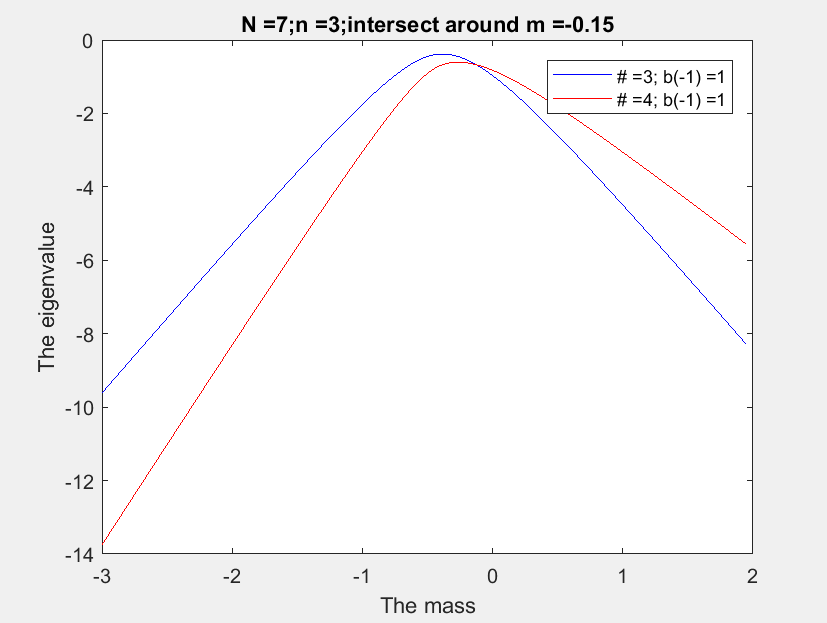
\includegraphics[scale=0.8]{subspinters.jpg}
\end{center}
In this simulation, we graph the eigenvalues of two invariant subspaces: one with the number of fermions equal to $3$ and $b_{-1} = s$, the other one with number of fermions equal to $4$ and $b_{-1} =s $. We definitely know that for $|m| \gg 0$, the ground state lies in one of these subspaces. But when exactly does the transition happen? I expect that if we find the point intersection for every $N$, then it will converge to the critical mass as $N \rightarrow \infty$.

The following chart shows the track of the point of intersection for different values of $N$. Unfortunately, for $N=13$, Matlab on my computer writes that he's out of memory (the size of the Hamiltonian is then $3\cdot 2^{13}  = 24,576$, so it contains $603,979,776$ entries.

\begin{center}
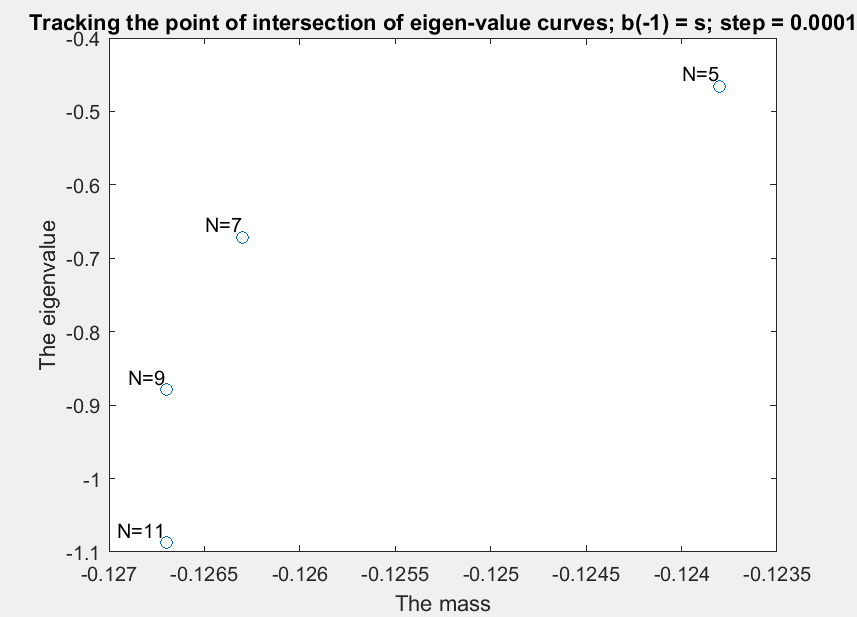
\includegraphics[scale=0.8]{track.jpg}
\end{center}
It seems that the bigger $N$ gets, the smaller step should be to distinguish the masses of intersection.

To distinguish $N= 9$ and $N=11$ cases, I also made a simulation for even a smaller step:
\begin{center}
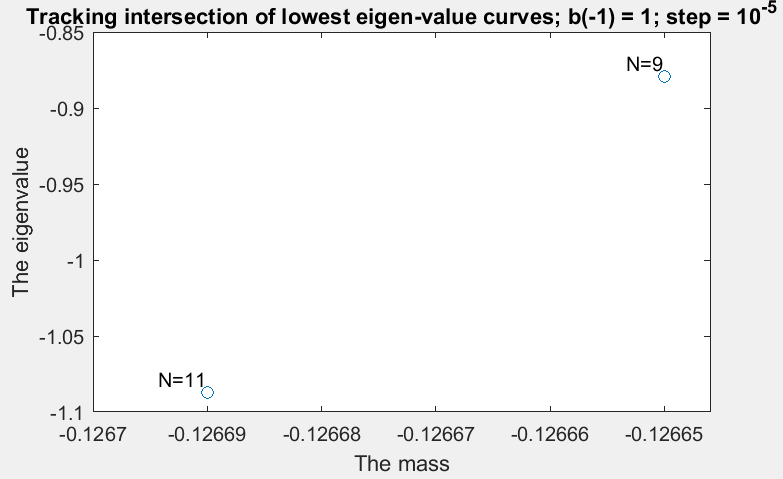
\includegraphics[scale=0.8]{track2.jpg}
\end{center}

In these simulations, I use only odd $N$. The reason is that then $|\gs\rangle$ lies in different invariant subspaces for $m \gg 0$ and $m \ll 0$, so there should be some value of mass when $|\gs\rangle$ transitions from one subspace to another. There's only one such subspace for even $N$ though.

\subsection{Wilson loop for $m \ll 0$}
The proofs are completely analogous to the ones for $m \gg 0$. Nevertheless, I include them for completeness.
\subsubsection{Estimate for $\lambda_1$}
\begin{proposition}
Let $\lambda_1$ be the lowest eigen-value of $H$, which is considered as a function of mass $m$. Then
\[
\lim_{m \rightarrow -\infty} \frac{\lambda_1}{m} = 2 \left[\frac{N+1}{2}\right] \sqrt{\frac{n}{2\pi}}.
\]
Also, for $m < 0$,
\[
\lambda_1(m) < 2m \left[\frac{N+1}{2}\right] \sqrt{\frac{n}{2\pi}}
\]
(note:the inequality is strict!). The limit implies that for $m \ll 0$ and $N$ large, the lowest energy level can be approximated as
\[
\lambda_1(m) \approx Nm \sqrt{\frac{n}{2\pi}}
\]
\end{proposition}
Probably a subtle moment in the proof in contrast to $m > 0$ case is that 
\[\min_{\|\psi\| = 1} 2m\sqrt{\frac{n}{2\pi}} \langle \psi | D|\psi\rangle = 2m\sqrt{\frac{n}{2\pi}}\max_{\|\psi\| = 1}  \langle \psi | D|\psi\rangle = 2m\sqrt{\frac{n}{2\pi}}\langle \st_1(s) | D|\st_1(s)\rangle =  2m\sqrt{\frac{n}{2\pi}}\left[\frac{N+1}{2}\right]\]
where $m < 0$ is assumed.
\begin{proof}
For $m < 0$, we see that
\[
m^{-1}\langle \st_1(s)|H|\st_1(s)\rangle < m^{-1} \langle \gs |H|\gs \rangle = m^{-1} \min_{\|\psi\|=1} \langle \psi |H|\psi\rangle \leq m^{-1} \min_{\|\psi\|=1} \langle \psi|A|\psi\rangle + 2\sqrt{\frac{n}{2\pi}} \langle \st_1(s)|D|\st_1(s)\rangle,
\]
where the last inequality is obtained from the principle that the minimum of the sum is greater than or equal to the sum of minimums (but then, we multiply by a negative mass, so the inequality flips). Note:
\[
\langle \st_1(s)|H|\st_1(s)\rangle = 2m \sqrt{\frac{n}{2\pi}} \langle \st_1(s)|D|\st_1(s)\rangle = 2m \left[\frac{N+1}{2}\right] \sqrt{\frac{n}{2\pi}},
\]
which, together with the first chain of inequalities, show that (remember: for $m < 0$!)
\[
\lambda_1(m) < 2m \left[\frac{N+1}{2}\right] \sqrt{\frac{n}{2\pi}}.
\]
Now, taking the limit as $m \rightarrow -\infty$ in the first sequence of inequalities proves that
\[
\lim_{m \rightarrow -\infty} \frac{\lambda_1}{m} = 2 \left[\frac{N+1}{2}\right] \sqrt{\frac{n}{2\pi}}.\qedhere
\]
\end{proof}

\subsubsection{Ground states}

\begin{lemma} \label{l:gs_conv_neg}
The following hold:
\begin{enumerate}
\item For any basic ket $|\psi\rangle$ such that $\langle \psi |D|\psi\rangle < [(N+1)/2]$ (i.e., $|\psi\rangle \neq |\st_1(i)\rangle$ for any $i$), we have $\lim_{m \rightarrow -\infty} \langle \gs | \psi \rangle = 0$;
\item For\footnote{By this I mean that there exists $m_0 < 0$ such that for all $m \leq m_0$ the statement is true.} $m \ll 0$ we have $\left\langle \gs | \st_1(s) \right\rangle \neq 0$. In particular, if for every low enough mass we choose $|\gs\rangle$ so that $\langle \gs | \st_1(s) \rangle > 0$ (which is possible), then $\lim_{m \rightarrow -\infty} |\gs\rangle = |\st_1(s)\rangle$. 
\item As a consequence of the above, for $m \ll 0$, $|\gs\rangle \in P_s$, and the number of fermions in each non-zero component of $|\gs\rangle$ is equal to $[(N+1)/2]$.
\end{enumerate}
\end{lemma}
\begin{proof}
\begin{enumerate}
\item Indeed, we see that
\[
\langle \psi | \gs \rangle = \frac{1}{\lambda_1} \langle \psi | H|\gs\rangle = \frac{1}{\lambda_1} \langle \psi |A|\gs\rangle + \frac{2m}{\lambda_1} \sqrt{\frac{n}{2\pi}} \langle \psi | D | \gs \rangle = \frac{1}{\lambda_1} \langle \psi |A|\gs\rangle + \frac{2m}{\lambda_1} \sqrt{\frac{n}{2\pi}} \cdot a \langle \psi | \gs \rangle
\]
where $a$ is an eigen-value of $D$ (which is not equal to $[(N+1)/2]$ by assumption). The above can be rewritten as
\[
\langle \psi | \gs\rangle = \frac{1}{\lambda_1} \frac{1}{1- \frac{2ma}{\lambda_1}\sqrt{\frac{n}{2\pi}} } \langle \psi | A | gs\rangle.
\]
We see that 
\[
1- \frac{2ma}{\lambda_1}\sqrt{\frac{n}{2\pi}} \rightarrow 1 - a [(N+1)/2]^{-1} \neq 0
\]
therefore
\[
\lim_{m \rightarrow -\infty}\langle \psi | \gs \rangle = 0.
\]
\item Since each $P_i$ is invariant under $H$, we find $j$ such that $|\gs \rangle \in P_j$, so we can write it as $|\gs\rangle = \alpha |\st_1(j)\rangle + |v\rangle$, where $|v\rangle \perp |\st_1(j)\rangle$. The first part of the lemma, together with $\langle \gs | \gs \rangle = 1$, implies
\[
\lim_{m \rightarrow \-\infty} (1 - |\alpha|^2) = 0
\]
or $\lim_{m \rightarrow -\infty} |\langle \gs |\st_1(j)\rangle| = 1$. If we made the choice of ground states so that $\alpha > 0$, then $\lim_{m\rightarrow -\infty} \alpha = 1$, so $|\gs\rangle \rightarrow |\st_1(j)\rangle$.

Let's prove that $j = s$. Write $|\gs\rangle = \alpha |\st_1(j)\rangle + \beta |v\rangle$ and $|\gs^\prime\rangle = \alpha |\st_2(s)\rangle + \beta |v^\prime \rangle$. The vector $|v^\prime \rangle$ is totally the same as $|v\rangle$ except that we substitute everywhere the bosonic state $b_{-1} = j$ with the state $b_{-1} = s$. The constants $\alpha$ and $\beta$ can be chosen real, $\alpha > 0$, and $\alpha^2+\beta^2 = 1$. Then we compare the expectation values of the Hamiltonian:
\[
\langle \gs | H|\gs \rangle  = \alpha^2 \left(2m\left[\frac{N+1}{2}\right] \sqrt{n/2\pi} + \left[\frac{N}{2}\right](j-s+1)^2 + \left[\frac{N-1}{2}\right] (j-s)^2 \right) + O(\beta),
\]
\[
\langle \gs^\prime | H|\gs^\prime \rangle  = \alpha^2 \left(2m\left[\frac{N+1}{2}\right] \sqrt{n/2\pi} + \left[\frac{N}{2}\right]\right) + O(\beta),
\]
hence their difference is
\[
\langle \gs | H|\gs \rangle - \langle \gs^\prime | H|\gs^\prime \rangle = \alpha^2\left((\left[\frac{N}{2}\right]-1)(j-s+1)^2 + \left[\frac{N-1}{2}\right] (j-s)^2\right) + O(\beta).
\]
It is supposed to be always negative (because of the definition of the ground state). However, we can make $O(\beta)$ as small as we want, whereas $\alpha^2$ tends to $1$ and is multiplied by something stubbornly positive. Therefore, the difference can stay negative iff $j = s$.
\end{enumerate}
\end{proof}

\begin{proposition}\label{p:low_mass_nondeg}
For $m \ll 0$, a ground state is non-degenerate.
\end{proposition}
\begin{proof}
Assume on the contrary that it is degenerate for $m \ll 0$. This means there's a sequence of values of masses $m_k \rightarrow \infty$ and sequences of ground states $|\gs_k\rangle$ and $|\gs^\prime_k\rangle$ such that $\langle\gs_k^\prime|\gs_k\rangle = 0$. However, passing to the limit in the slots of the Hermitian product yields $\langle \st_1(s) | \st_1(s) \rangle \neq 0$. This is a contradiction, and thus the ground state is unique for sufficiently low $m$.
\end{proof}

\begin{proposition}
Let $\Sigma = N^{-1}\sum \langle E_{l,l+1} \rangle$ be the electric field operator. Then\footnote{No matter how we choose the ground states for every value of mass since we're under the Hermitian inner product.} 
\[
\lim_{m \rightarrow -\infty} \Sigma = \frac{1}{N}\left[\frac{N}{2}\right].
\]
\end{proposition}
\begin{proof}
Indeed, by Lemma \ref{l:gs_conv_neg} we can assume that $\lim_{m \rightarrow \infty} |\gs\rangle = |\st_2(s)\rangle$. Then 
\[
\langle \gs |\Sigma | \gs \rangle \rightarrow \frac{1}{N}\sum_l\langle \st_1(s) | E_{l,l+1}|\st_1(s)\rangle = \frac{1}{N}\left[\frac{N}{2}\right] \approx 0.5.\qedhere
\]
\end{proof}
\noindent \textbf{Remark.} This contradicts numerical simulation by Ercolessi \cite{ercolessi}. They obtained that $\Sigma \rightarrow \approx 0.7$. We don't understand why.

\subsection{Conjectures}

\begin{conj}
There is a phase transition.
\end{conj}

\begin{conj}
For every $N$ odd, let $\hat{m}(N)$ be the mass at which the lowest eigen-value curves of the restrictions of $H$ to the subspaces with $b_{-1} = s$ and number of fermions respectively $[N/2]$ and $[(N+1)/2]$ intersect. Let $\hat{m} = \lim_{N \rightarrow \infty} \hat{m}(N)$. Then there's a phase transition of $\hat{m}$.
\end{conj}

\begin{conj}
For $N$ even, the ground state is non-degenerate and $|\gs\rangle$ can be chosen continuously as a function of $m$. For $N$ odd, there is a unique value of mass at which the ground state is degenerate.
\end{conj}

%To show that the aforementioned transition happens, it STS that the only two possible invariant subspace (with respect to the number of fermions and the value of $b_{-1}$) that $|\gs\rangle$ can reside in are determined by $[N/2]$ and $[(N+1)/2]$. 

%\subsection{Numerical records}
%For $n = 9$, $N = 6$, the space given by $3$ fermions and $b_{-1} = 4$ is $C_6^3 = 20$ dimensional. For $m = 0$ checked that all $20$ vectors are in the decomposition of $|\gs\rangle$. For $m=1$, I can say there are $19$ vectors. For $m = 10$, there are $12$ vectors.